\documentclass[11pt,a4paper]{article}
\usepackage[a4paper,margin=2.3cm]{geometry}
\usepackage{amsmath,amssymb,amsthm}
\usepackage{booktabs}
\usepackage{graphicx}
\usepackage{float}
\usepackage[numbers]{natbib}
\usepackage{hyperref}
\usepackage{xcolor}
\usepackage{enumitem}
\usepackage{array}
\usepackage{longtable}
\usepackage{caption}
\usepackage{url}
\graphicspath{{figures/}{figures/peak_shaving_diagnostics/}{figures/peak_shaving_submission/}{figures/peak_shaving_smpt/}{./}}
\hypersetup{colorlinks=true,linkcolor=blue,citecolor=blue,urlcolor=blue}
\captionsetup{font=small}
\setlength{\emergencystretch}{3em}

\newtheorem{proposition}{Proposition}
\newtheorem{remark}{Remark}
\newtheorem{assumption}{Assumption}
\newtheorem{definition}{Definition}
\newcommand{\qos}{q}
\newcommand{\T}{\mathcal{T}}
\newcommand{\M}{\mathcal{M}}
\newcommand{\D}{D}
\newcommand{\w}{\boldsymbol{w}}
\newcommand{\p}{\boldsymbol{p}}
\newcommand{\g}{\boldsymbol{g}}

\title{\textbf{A Simulation-Based Study of Time-of-Use Pricing for Fixed-Capacity Inference Services:\\
Provider Competition, QoS Protection, and the Profit Boundary}}
\author{Anonymous Author}
\date{}

\begin{document}
\maketitle

\begin{abstract}
Large language model (LLM) inference services operate under short-run fixed graphics processing unit (GPU) capacity, while time-varying arrivals can create costly off-peak idleness and peak quality-of-service (QoS) degradation. This paper develops an auditable simulation model to test whether time-of-use pricing can shift time-flexible inference demand away from congested periods and protect QoS without capacity expansion. The model combines two heterogeneous inference providers, one application programming interface (API) intermediary, time-rigid and time-flexible users, direct access, and an outside option. Provider prices use a low-dimensional time-shape family, and provider competition is approximated through fictitious play with finite-grid regret checks. Verification uses fixed-point residuals and solver traces; validation is bounded to public price scales and controlled vLLM overload measurements. In the congested uniform-pricing baseline, peak utilization is $0.782$ and minimum QoS is $0.756$. Dynamic coarse-grid and fine-grid snapshots reduce peak utilization to $0.706$ and $0.666$, respectively, and raise minimum QoS to $0.968$ and $0.990$. A double-oracle mixed-strategy check on the full 225-point grid gives a $5\times5$ support profile with maximum regret $0.203$, expected peak utilization $0.703$, and minimum QoS $0.970$. Additional baselines and stress checks indicate that QoS gains are more reproducible than profit gains. Profit is unstable across solver objects: the coarse snapshot gives $+9.3\%$, the fine snapshot gives $-1.9\%$, and the low-regret mixed profile gives about $-2.8\%$. The results support time-of-use pricing as a QoS-protection instrument under fixed capacity, not as a reliable profit-improvement mechanism.
\end{abstract}

\noindent\textbf{Keywords:} inference-service simulation; time-of-use pricing; peak shaving; fixed capacity; QoS protection; verification and validation; finite-grid regret

\section{Introduction}
\label{sec:intro}

Large language model (LLM) inference has shifted from offline batch processing to continuously operating online services. Interactive chat, code generation, agentic workflows, scheduled evaluation, and periodic batch jobs exhibit different intraday arrival patterns. As a result, graphics processing unit (GPU) inference clusters experience pronounced peak--valley load variation that cannot be eliminated easily by short-run capacity expansion \cite{crankshaw2017clipper,gujarati2020clockwork,yu2022orca,kwon2023pagedattention,agrawal2024sarathiserve}. When utilization approaches a local capacity threshold, time to first token (TTFT), queueing delay, and completion rates may deteriorate rapidly. Quality-of-service (QoS) degradation then reduces the volume of requests that can be completed and billed, while also lowering user satisfaction.

This study focuses on a fixed-capacity operating regime. GPU procurement and deployment require lead time and involve sunk costs, and idle off-peak capacity still incurs holding costs. An operational alternative to immediate expansion is to use prices as a demand-shaping instrument. Peak-period prices are raised, off-peak prices are lowered, and time-flexible demand is encouraged to move toward periods with spare capacity. The motivation is related to real-time electricity pricing and demand response \cite{schweppe1988spot,borenstein2005long,albadi2008summary,faruqui2010household,siano2014demand}; however, the engineering mechanism is different. Inference-service quality is governed by local GPU utilization, latency, and completion rates, rather than by generation constraints or power-flow equations.

Inference-service markets also differ from the single-platform monopoly commonly used in simplified pricing models. The same open-source model family, such as GLM, can be deployed by multiple providers. When user-visible model capability is approximately homogeneous, competition is driven primarily by price, available capacity, and realized QoS. Provider capacity is also heterogeneous. A smaller provider may enter congestion earlier when an intermediary routes traffic to it. These observations motivate the simulated market used in this paper: two capacity-heterogeneous providers, one routing intermediary, direct-provider access, and an outside option.

The main gap is not the absence of another pricing heuristic. It is the absence of a reproducible simulation model that places congestion-sensitive QoS, provider competition, intermediary routing, direct-provider choice, and market exit in the same fixed-capacity setting. The closest modelling template comes from electricity demand-response studies, where time-varying prices are tested through explicit demand, utility, load, and welfare calculations. The present paper adapts that style of modelling and numerical reporting to inference services while keeping the engineering mechanism distinct.

The study makes three contributions. First, it formulates a fixed-capacity simulation model of time-of-use inference pricing with two competing heterogeneous providers, one routing intermediary, time-rigid and time-flexible users, and an outside option. The model jointly represents idle-capacity holding costs, QoS degradation under congestion, and time-shifting of user demand. Second, it uses a low-dimensional pricing-shape family and fictitious play to obtain reproducible candidate responses. Naive best-response dynamics cycle in the congested regime, whereas fictitious play produces time-averaged strategies. Finite-grid regret is reported to state how strong the equilibrium approximation is. Third, it separates the QoS result from the profit result through solver checks, service-management baselines, structural ablations, fixed-policy stress tests, and restricted local re-solves. These checks support a bounded QoS-protection claim in the congested setting, but they do not support a stable profit-improvement claim. The paper positions time-of-use pricing as a service-quality management tool rather than a general revenue-enhancement mechanism.

\section{Related Work and Modelling Positioning}
\label{sec:related}

\subsection{Inference serving and QoS-aware market simulation}

Online inference-serving research explains why QoS is sensitive to utilization. Prior systems have studied low-latency serving, batching, memory management, model parallelism, prefill/decode separation, and serving simulators \cite{crankshaw2017clipper,gujarati2020clockwork,romero2021infaas,yu2022orca,li2023alpaserve,sheng2023flexgen,kwon2023pagedattention,agrawal2024sarathiserve,patel2024splitwise,zhong2024distserve,agrawal2024vidur}. These studies motivate the local QoS-degradation function used here. They do not usually model user exit, intermediary routing, direct-provider choice, and competing provider prices within one market-level simulation.

Recent AI-service market studies have begun to analyse inference costs, menu pricing, token-capacity contracts, and Stackelberg-style GPU-service pricing \cite{demirer2025emerging,erdil2025inference,bergemann2025menu,guo2026prillm,yan2026stackelberg,cunningham2026token,liu2026locational}. This paper is narrower. It does not estimate a production demand curve or solve a general continuous pricing game. Its contribution is a verifiable simulation setting in which price timing, QoS feedback, routing, and exit can be examined together.

\subsection{Electricity dynamic pricing as a structural template}

Electricity pricing provides the closest precedent for using prices to reshape time-varying demand under short-run capacity limits. Spot pricing and real-time pricing studies treat price as a scarcity signal and examine how demand response changes load profiles, efficiency, and consumer or producer surplus \cite{schweppe1988spot,borenstein2005long,allcott2011rethinking}. Survey and experimental work further show that household response differs across real-time, time-of-use, and critical-peak designs \cite{albadi2008summary,faruqui2010household,siano2014demand}.

The mathematical style of this literature is useful for the present paper. Utility-maximization and demand-response models first specify user utility and demand, then define the supplier or system objective, and finally report peak-load, welfare, and sensitivity checks \cite{samadi2010optimal,yang2013game,yu2016supply,srinivasan2017game}. The same ordering is adopted here: Sections~\ref{sec:model}--\ref{sec:setup} define agents, utilities, loads, QoS, profit, candidate strategies, solver checks, and reported metrics before the results are interpreted.

The analogy is limited. Electricity systems are governed by generation, network, and reliability constraints. Inference services are governed by local GPU serving capacity, queueing, time-to-first-token, completion rates, and API routing. The model borrows the demand-response reporting structure, not the physical equations of a power system.

\subsection{Congestion pricing, revenue management, and platform choice}

The paper also draws on congestion pricing and revenue-management work, where prices allocate scarce capacity under time-varying demand \cite{vickrey1969congestion,arnott1990bottleneck,gallego1994dynamic,elmaghraby2003dynamic,bitran2003overview,talluri2004revenue,phillips2005pricing}. In contrast with a single monopolist model, the present setting includes two providers, one intermediary, direct-provider options, and an outside option. User choice is represented through standard discrete-choice and platform-market tools \cite{mcfadden1974conditional,anderson1992discrete,train2009discrete,rochet2003platform}. This modelling choice matters for the main result: QoS can improve while profit remains unstable because users and surplus can move across channels or leave the market.

\section{Simulation Model}
\label{sec:model}

\subsection{Market structure and sequence of decisions}

A day is divided into $T$ periods, $\T=\{1,\ldots,T\}$, each of length $h$. The simulated market contains the following agents:
\begin{itemize}[leftmargin=2em]
  \item \textbf{Two heterogeneous inference providers} $\M=\{A,B\}$ with fixed capacities $G_A>G_B$. Both deploy the same open-source model and are treated as nearly homogeneous in model capability. Provider $m$ chooses a period-specific wholesale price $w_{m,t}$ for the intermediary and a period-specific direct retail price $p^D_{m,t}$ for users.
  \item \textbf{One API intermediary} that observes wholesale prices and chooses a period-specific retail price $p_t$ and routing weights $r_{m,t}$, where $\sum_m r_{m,t}=1$.
  \item \textbf{Two user types} who choose among the intermediary channel, direct access to provider $A$, direct access to provider $B$, and an outside option according to a logit random-utility model.
\end{itemize}
The sequence, summarized in Figure~\ref{fig:market_schematic}, is: providers post prices simultaneously in a Nash-pricing stage, the intermediary computes its best response, and user choices and QoS are determined through a congestion fixed point.

\begin{figure}[H]
\centering
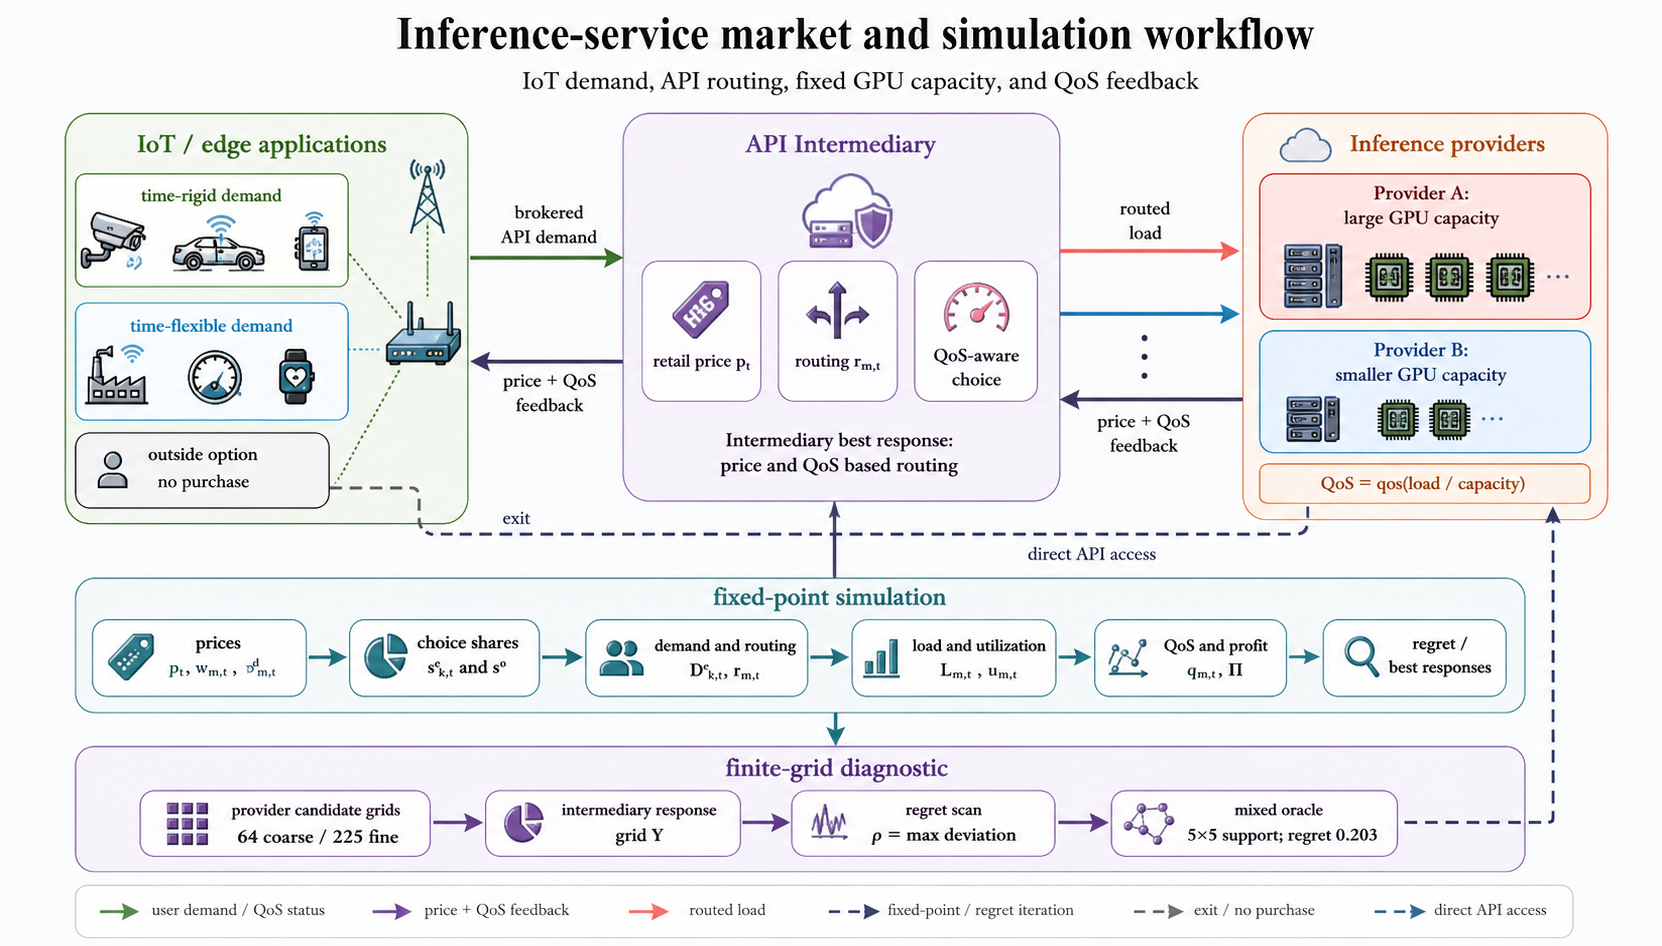
\includegraphics[width=\textwidth]{market_schematic_iot_imagegen_2026-06-22.png}
\caption{Market structure and simulation workflow. Users may buy through the API intermediary, connect directly to a provider, or exit. The intermediary routes traffic between two providers on the basis of prices and QoS. The lower bands summarize the demand--routing--load--QoS fixed point and the finite-grid equilibrium diagnostic used to evaluate candidate pricing strategies.}
\label{fig:market_schematic}
\end{figure}

\subsection{User choice and the outside option}

There are two user types, $\theta\in\{R,E\}$. Type $R$ users are time-rigid, whereas type $E$ users are time-flexible. For channel $k$ and period $t$, deterministic utility is defined as
\begin{equation}
  z^\theta_{k,t}=\log b_k+\log a_t
  -\alpha_\theta\!\left[\text{price}_{k,t}+c_s^\theta(1-\pi^\theta_t)-p_0\right]
  -\gamma(1-q_{k,t}).
  \label{eq:utility}
\end{equation}
Here $b_k$ denotes channel brand value or convenience, $a_t$ denotes period preference, $\pi^\theta_t$ is the native-period distribution for type $\theta$, and $q_{k,t}$ is channel QoS. Switching cost is represented in price-equivalent units and is scaled by the same price-sensitivity parameter $\alpha_\theta$. The two user types differ only through parameters. Time-rigid users have lower price sensitivity, higher switching cost, and a native-period distribution concentrated in peak periods. Time-flexible users have higher price sensitivity, lower switching cost, and a more dispersed native-period distribution.

The logit denominator includes a no-purchase outside option with deterministic utility $u_0$. The share of type $\theta$ users choosing channel $k$ in period $t$, and the corresponding exit probability, are
\begin{equation}
  s^\theta_{k,t}=\frac{\exp(z^\theta_{k,t})}{\exp(u_0)+\sum_{k',t'}\exp(z^\theta_{k',t'})},
  \qquad
  s^\theta_0=\frac{\exp(u_0)}{\exp(u_0)+\sum_{k',t'}\exp(z^\theta_{k',t'})}.
  \label{eq:share}
\end{equation}
The internal shares sum to less than one; the remaining mass $s^\theta_0$ is interpreted as genuine market exit and is not reallocated across the purchasable options. Consequently, a price increase may reduce internal demand rather than merely redistributing it among providers or channels.

\subsection{Demand, load, and QoS}

Demand from type $\theta$ users for channel $k$ consists of an elastic component and a rigid/replay component. Both components are allocated by the channel's own choice share, which prevents the total rigid quantity in a period from scaling with the number of available channels:
\begin{equation}
  \D^\theta_{k,t}=\bar F_\theta\,m^\theta(\p,q)\,s^\theta_{k,t}
  +\bar R^\theta_t\,\sigma[\beta(v_r-\text{price}_{k,t})]s^\theta_{k,t}.
  \label{eq:demand}
\end{equation}
Here $\sigma(x)=(1+\exp[-x])^{-1}$. In the implementation, the elastic market-size multiplier is
\begin{equation}
  m^\theta(\p,q)
  =
  1+\eta\,[p_0-\bar p_\theta(\p,q)]_+,
  \qquad
  \bar p_\theta(\p,q)
  =
  \frac{\sum_{k,t}s^\theta_{k,t}(\p,q)\,\text{price}_{k,t}}
       {\sum_{k,t}s^\theta_{k,t}(\p,q)} ,
  \label{eq:market_size}
\end{equation}
with $\eta=1.2$ in the main calibration. The rigid/replay response uses $v_r=1.80$ and $\beta=5.0$ in the main calibration. Total demand is the population-weighted sum over the two types, with weights $(\pi_R,\pi_E)$. The model is not a fixed-total-demand model. The outside option allows internal demand to contract, and the elastic market-size term allows demand to expand at lower prices. The later discussion of the profit boundary is a numerical decomposition, not a theorem based on fixed total demand.

Provider $m$'s load in period $t$ equals direct demand plus the intermediary demand routed to that provider:
\begin{equation}
  L_{m,t}=\D^D_{m,t}+r_{m,t}\D^I_t,
  \qquad
  u_{m,t}=L_{m,t}/G_m,
  \qquad
  q_{m,t}=\qos(u_{m,t}).
  \label{eq:load}
\end{equation}
The QoS degradation function $\qos(u)$ begins to decline once utilization exceeds a threshold $\bar u$. Since $G_B<G_A$, the smaller provider reaches the congested region earlier under the same incoming load. The main experiments use a smooth sigmoid-type degradation shape, while threshold, linear, and square-root shapes are retained as robustness checks in the artifact set. For a fixed routing matrix, the QoS fixed point is computed by damped iteration:
\begin{equation}
  \tilde q^{(n+1)}_{m,t}
  =\qos\!\left(\frac{L_{m,t}(q^{(n)})}{G_m}\right),
  \qquad
  q^{(n+1)}_{m,t}
  =(1-\lambda)q^{(n)}_{m,t}+\lambda \tilde q^{(n+1)}_{m,t},
  \label{eq:qos_fixed_point}
\end{equation}
with damping $\lambda=0.35$, stopping tolerance $10^{-9}$, and a 200-iteration limit in the reported implementation.

\subsection{Profit with fixed-capacity holding cost}

Provider $m$'s profit is wholesale revenue plus direct retail revenue, minus fixed capacity holding cost and QoS degradation cost:
\begin{equation}
  \Pi_m=h\!\sum_t\! w_{m,t}r_{m,t}\D^I_t q_{m,t}
  +h\!\sum_t\! p^D_{m,t}\D^D_{m,t}q_{m,t}
  -h\!\sum_t\! c_g G_m
  -h\!\sum_t\! c_q(1-q_{m,t})L_{m,t}.
  \label{eq:firm_profit}
\end{equation}
The holding cost $c_gG_m$ is charged on fixed capacity rather than on realized utilization. It gives providers an incentive to fill off-peak capacity by lowering prices in low-load periods. This specification distinguishes the present model from formulations that treat capacity only as a fixed upper bound and ignore the cost of idle resources.

The intermediary's channel QoS and average wholesale cost are
\begin{equation}
  q^I_t=\sum_m r_{m,t}q_{m,t},
  \qquad
  \bar w_t=\sum_m r_{m,t}w_{m,t}.
  \label{eq:intermediary_channel}
\end{equation}
Its profit is retail revenue minus wholesale cost and QoS degradation cost:
\begin{equation}
  \Pi_I
  =h\sum_t p_t\D^I_t q^I_t
  -h\sum_t \bar w_t\D^I_t q^I_t
  -h\sum_t c_q(1-q^I_t)\D^I_t .
  \label{eq:intermediary_profit}
\end{equation}
System profit is
\begin{equation}
  \Pi^{\mathrm{sys}}=\Pi_I+\sum_{m\in\M}\Pi_m .
  \label{eq:system_profit}
\end{equation}

\section{Solution Method and Simulation Diagnostics}
\label{sec:solver}

\subsection{Low-dimensional pricing-shape family}

If each provider directly optimized $2T$ continuous prices, comprising period-specific wholesale and direct retail prices, the Nash game would be high-dimensional, non-convex, and difficult to reproduce numerically. Provider prices are restricted to a low-dimensional time-shape family:
\begin{equation}
  w_{m,t}=\bar w_m\big(1+\delta_m\widehat{\ell}_t\big),
  \qquad
  p^D_{m,t}=\bar p^D_m\big(1+\delta^D_m\widehat{\ell}_t\big).
  \label{eq:shape}
\end{equation}
The vector $\widehat{\ell}_t$ is a zero-mean normalized load shape obtained from the rigid-demand baseline and treated as exogenous. Each provider strategy is represented by four scalars, $(\bar w_m,\delta_m,\bar p^D_m,\delta^D_m)$. A value of $\delta_m=0$ gives uniform pricing, while $\delta_m>0$ raises prices during peak periods. This parameterization sacrifices global optimality in the full continuous price space, but it improves transparency, repeatability, and numerical control. All equilibrium language in this paper refers to the pricing-shape family unless explicitly stated otherwise; no claim is made about a global optimum in the unrestricted $2T$-dimensional strategy space. Table~\ref{tab:solver_grids} reports the finite grids used by the solver.

\begin{table}[H]
\centering
\caption{Finite candidate grids used by the solver diagnostics}
\label{tab:solver_grids}
\small
\begin{tabular}{p{0.23\textwidth}p{0.37\textwidth}p{0.29\textwidth}}
\toprule
Grid object & Candidate values & Role in the paper \\
\midrule
Provider coarse grid &
$\bar w\in\{0.30,0.85\}$, $\delta\in\{-0.4,-0.133,0.133,0.4\}$, $\bar p^D\in\{0.70,1.50\}$, $\delta^D\in\{-0.4,-0.133,0.133,0.4\}$ &
64 strategy shapes per provider for the coarse fictitious-play diagnostic. \\
Provider fine grid &
$\bar w\in\{0.27,0.575,0.88\}$, $\delta\in\{-0.4,-0.2,0,0.2,0.4\}$, $\bar p^D\in\{0.60,1.10,1.60\}$, $\delta^D\in\{-0.4,-0.2,0,0.2,0.4\}$ &
225 strategy shapes per provider for the fine snapshot and mixed-oracle scan. \\
Intermediary grid &
$\bar p\in\{0.60,0.80,1.10,1.60\}$, $\delta_p\in\{-0.2,0,0.2\}$, $\beta_r\in\{1.5,4.0\}$ &
Retail price and routing response grid evaluated for every provider candidate pair. \\
\bottomrule
\end{tabular}
\end{table}

\subsection{Candidate evaluation and finite-game equilibrium certificate}

Let $s_m=(\bar w_m,\delta_m,\bar p^D_m,\delta^D_m)$ denote provider $m$'s pricing-shape strategy, and let $\mathcal S_m$ be the finite candidate grid used in a given diagnostic. For any candidate pair $(s_A,s_B)$, Eq.~(\ref{eq:shape}) gives wholesale and direct prices. The intermediary then chooses a retail-price shape and a routing sensitivity,
\[
  y=(\bar p,\delta_p,\beta_r)\in\mathcal Y ,
  \qquad
  p_t=\bar p\big(1+\delta_p\widehat{\ell}_t\big),
\]
where $\mathcal Y$ is the intermediary's finite response grid. Conditional on $y$, routing is updated as a logit response to wholesale prices and provider QoS:
\begin{equation}
  r_{m,t}
  =
  \frac{\exp[-\beta_r w_{m,t}+\omega q_{m,t}]}
       {\sum_{j\in\M}\exp[-\beta_r w_{j,t}+\omega q_{j,t}]},
  \qquad \omega=3 .
  \label{eq:routing_logit}
\end{equation}
Because routing depends on QoS and QoS depends on routed load, Eq.~(\ref{eq:routing_logit}) and Eq.~(\ref{eq:qos_fixed_point}) are solved as a joint damped fixed point during intermediary evaluation. The intermediary best response is
\begin{equation}
  y^\star(s_A,s_B)\in
  \arg\max_{y\in\mathcal Y}
  \Pi_I\big(s_A,s_B,y\big),
  \label{eq:intermediary_best_response}
\end{equation}
and the provider payoffs in the induced finite game are
\begin{equation}
  U_m(s_A,s_B)=
  \Pi_m\big(s_A,s_B,y^\star(s_A,s_B)\big).
  \label{eq:finite_game_payoff}
\end{equation}

A pure-strategy Nash equilibrium on the finite grid would require
\begin{equation}
  U_m(s_m^\star,s_{-m}^\star)
  \ge
  U_m(s_m,s_{-m}^\star)
  \quad
  \forall s_m\in\mathcal S_m,\quad m\in\M .
  \label{eq:pure_nash}
\end{equation}
The paper does not derive a closed-form Nash equilibrium because the payoff in Eq.~(\ref{eq:finite_game_payoff}) is generated by a non-linear QoS fixed point, a discrete intermediary response, and finite candidate grids. Instead, it reports exploitability through unilateral-deviation regret. For a pure candidate pair,
\begin{equation}
  \rho_m(s_A,s_B)
  =
  \max_{s'_m\in\mathcal S_m}U_m(s'_m,s_{-m})
  -U_m(s_m,s_{-m}),
  \qquad
  \rho(s_A,s_B)=\max_m\rho_m(s_A,s_B).
  \label{eq:pure_regret}
\end{equation}
For a mixed profile $\mu=(\mu_A,\mu_B)$ over the finite grids, expected payoff and regret are
\begin{align}
  \bar U_m(\mu_A,\mu_B)
  &=
  \sum_{i,j}\mu_A(i)\mu_B(j)\,U_m(s_A^i,s_B^j), \label{eq:mixed_payoff}\\
  \rho_A(\mu)
  &=
  \max_i\sum_j\mu_B(j)U_A(s_A^i,s_B^j)
  -\bar U_A(\mu_A,\mu_B), \nonumber\\
  \rho_B(\mu)
  &=
  \max_j\sum_i\mu_A(i)U_B(s_A^i,s_B^j)
  -\bar U_B(\mu_A,\mu_B). \label{eq:mixed_regret}
\end{align}
A zero-regret profile would be a mixed Nash equilibrium of the finite candidate game. The reported value $0.203$ is a finite-grid exploitability certificate, not a proof of equilibrium in the unrestricted continuous strategy space.

\subsection{Fictitious play and finite-grid regret}

Provider best responses are computed by grid search over the four pricing-shape parameters. Grid search is robust to non-smooth QoS responses, has a predictable computational budget, and facilitates independent replication. The intermediary response is also obtained by grid search. Each candidate evaluation embeds a joint fixed point over routing and QoS, which is solved by damped iteration. A deeper nested continuous optimizer is not used because it substantially increases computational cost in the congested regime.

Naive best-response iteration, in which providers alternately best-respond to the opponent's current strategy, produces cyclic behaviour in the congested regime. Strategies repeatedly switch between two configurations, generating a limit cycle. The solver therefore uses fictitious play: each provider best-responds to the opponent's running average strategy rather than only to the most recent strategy. The resulting object is not an unrestricted pure-strategy Nash equilibrium. It is a time-averaged fictitious-play strategy within the pricing-shape family. It is treated as an acceptable equilibrium approximation only when the maximum profitable unilateral deviation, or regret, is sufficiently low. Parameter drift is not used as the primary convergence criterion, because it can give a false impression of convergence on a coarse grid.

For the fine grid, an additional double-oracle check is used. The procedure starts from a small candidate set and repeatedly adds best deviations against the current mixed profile on the complete 225-point fine grid. It then solves an empirical mixed profile on the restricted support by fictitious play and scans the full grid to compute regret.

\paragraph{Algorithmic outline.}
The reported solver follows five deterministic steps. First, construct the provider candidate grids and the intermediary response grid in Table~\ref{tab:solver_grids}. Second, for each provider candidate pair, enumerate intermediary responses, solve the joint routing--QoS fixed point, and select the intermediary response that maximizes Eq.~(\ref{eq:intermediary_profit}). Third, use the induced provider payoff matrix in Eq.~(\ref{eq:finite_game_payoff}) to run fictitious play on the coarse or fine grid. Fourth, compute pure-regret values using Eq.~(\ref{eq:pure_regret}) rather than treating parameter drift as convergence. Fifth, for the fine-grid mixed check, build a restricted support by double oracle and scan all 225 candidate strategies for each provider to obtain the mixed-regret certificate in Eq.~(\ref{eq:mixed_regret}). This outline plays the same role as the solution-algorithm block in electricity demand-response pricing papers, but every step here is evaluated through the inference-service QoS fixed point.

\begin{remark}[Solver verification and evidence boundary]
In the uncongested regime, QoS is identically one, the fixed point converges in one step, and grid search is deterministic; the cross-seed relative standard deviation of system profit is $4.31\times10^{-4}$. The congested regime requires a separate solver check. On the coarse grid, fictitious-play regret decreases monotonically from $133.6$ to $63.7$ and eventually to $4.98$, reaching regret $<5$ after 22 rounds. In the fine-grid pure snapshot, regret reaches a local minimum of approximately $14$ around round 10 and then increases, drifting to approximately $22$ after 40 rounds. The added double-oracle mixed check obtains a $5\times5$ support profile on the complete 225-point fine grid, with final maximum regret $0.203$. The QoS improvement is supported as a low-exploitability result for a finite-grid mixed/averaged strategy. It is not a theorem for the unrestricted continuous strategy space.
\end{remark}

\section{Verification, Validation, and Credibility Boundaries}
\label{sec:vv}

The simulation is deterministic conditional on the reported grids, parameter settings, and solver seeds. Verification asks whether the implementation follows the accounting, routing, and fixed-point equations used in Sections~\ref{sec:model}--\ref{sec:solver}. Validation asks a narrower question: whether the abstractions are credible enough for a mechanism study of fixed-capacity inference pricing. These checks bound the claims; they do not certify a production inference service or a real platform market.

\subsection{Implementation verification}

The implementation keeps the market equations, fixed-point QoS update, intermediary response, and provider candidate search in separate modules. The main verification checks are artifact based. In the uncongested setting, QoS is one and the degradation function is inactive, which verifies the below-threshold branch of the QoS model. Cross-seed runs in this regime give relative standard deviation $4.31\times10^{-4}$ for system profit. In the congested setting, the reported artifacts store the static baseline, coarse and fine candidate responses, checkpoint traces, diagnostic figures, and mixed-strategy oracle output.

\begin{table}[H]
\centering
\caption{Fixed-point verification for the reported congested-policy states}
\label{tab:fixed_point_verification}
\small
\begin{tabular}{lccc}
\toprule
Policy state & Converged & Iterations & Final residual \\
\midrule
Static pricing with QoS routing & Yes & 52 & $8.32\times10^{-10}$ \\
Off-peak discount only & Yes & 32 & $8.23\times10^{-10}$ \\
Peak surcharge only & Yes & 34 & $9.71\times10^{-10}$ \\
Dynamic coarse & Yes & 33 & $8.52\times10^{-10}$ \\
Dynamic fine snapshot & Yes & 35 & $6.44\times10^{-10}$ \\
\bottomrule
\end{tabular}
\end{table}

Table~\ref{tab:fixed_point_verification} reports residual checks for the market states used in the main comparisons and in the SMPT baseline diagnostics. A separate initialization and damping audit covers three initial QoS levels and three damping factors for the static, dynamic coarse, and dynamic fine states. It converges in 24 of 27 rows. The dynamic coarse and fine rows converge in all 18 combinations. The three non-converged rows occur for the static congested baseline with damping $0.5$, where the residual remains about $0.312$ at the 200-iteration limit. The reported static baseline itself uses the default damping $\lambda=0.35$ and converges below $10^{-9}$. This audit does not exhaust every candidate evaluation in the grid search, but it verifies the fixed-point states used in the paper's reported policy comparisons and identifies the numerical boundary for the most congested static case.

\subsection{Validation and calibration boundary}

Public API prices are used only to check the scale of normalized prices. They are not used to estimate price elasticity, switching cost, or outside-option utility. Controlled vLLM overload measurements are used only to anchor the qualitative shape of the QoS degradation proxy. The measurements use one NVIDIA GeForce RTX 4090, two Qwen2.5 model sizes, short generations, five repeats per concurrency level, and a 0.5-second TTFT service-level-agreement threshold. They support the threshold-shaped QoS assumption that service remains healthy below a local utilization boundary and deteriorates after overload. They do not replace real arrival traces, production completion curves, multi-GPU serving measurements, long-context workloads, or user price-elasticity estimates.

The sensitivity evidence is separated into three layers. First, fixed-policy stress tests perturb capacity, price sensitivity, switching cost, and the QoS threshold. Second, a two-dimensional fixed-policy phase grid varies capacity scale and price-sensitivity scale. Third, a restricted local candidate re-solve is run for five selected perturbations using a small candidate set built from static, dynamic coarse, dynamic fine, off-peak-only, and peak-only shapes. The last layer is a re-solved simulation diagnostic, not a global equilibrium computation.

\section{Experimental Design}
\label{sec:setup}

The numerical study follows the reporting logic commonly used in electricity demand-response simulations. It defines load and capacity scenarios, specifies price-policy baselines, computes peak-load and service-quality metrics, and tests sensitivity around the main mechanism. Two capacity regimes are used. The uncongested regime checks whether time-of-use prices can move demand when QoS is not binding. The congested regime activates the QoS degradation function and tests whether demand shifting protects service quality under fixed capacity.

The simulated day has $T=8$ periods and $h=3$ hours per period. Baseline capacity is $G_A=1500$ and $G_B=600$. The congested setting tightens capacity to $G_A=300$ and $G_B=120$. Baseline population weights are $(\pi_R,\pi_E)=(0.6,0.4)$; the congested setting uses $(0.4,0.6)$ to increase peak pressure. All economic parameters are synthetic calibrations. Their numerical values are used to support mechanism analysis and are not interpreted as production forecasts. Table~\ref{tab:main_parameters} summarizes the main parameters needed to reproduce the reported experiments.

\begin{table}[H]
\centering
\caption{Main simulation parameters used in the reported experiments}
\label{tab:main_parameters}
\small
\begin{tabular}{p{0.25\textwidth}p{0.23\textwidth}p{0.42\textwidth}}
\toprule
Parameter & Value & Interpretation \\
\midrule
$T,h$ & 8 periods, 3 hours & One simulated day. \\
$G_A,G_B$ & 1500, 600; congested 300, 120 & Fixed GPU serving capacities of providers A and B. \\
$(\pi_R,\pi_E)$ & baseline $(0.6,0.4)$; congested $(0.4,0.6)$ & Population weights for time-rigid and time-flexible users. \\
$\alpha_R,\alpha_E$ & 2.0, 5.0 & Price sensitivities in the logit utility. \\
$c_s^R,c_s^E$ & 0.60, 0.10 & Time-shifting costs in price-equivalent units. \\
$p_0,v_r,\eta$ & 0.80, 1.80, 1.2 & Baseline price, rigid/replay reservation value, and elastic market-growth slope. \\
$\bar u,\gamma,c_q$ & 0.82, 1.0, 0.35 & QoS threshold, QoS utility weight, and QoS degradation cost. \\
$c_g,u_0$ & 0.015, 0.0 & Fixed capacity holding cost and outside-option utility. \\
\bottomrule
\end{tabular}
\end{table}

The experimental design has four evidence layers. The first compares uniform pricing with dynamic candidate responses in uncongested and congested regimes. The second reports solver diagnostics, including pure-strategy regret and the finite-grid mixed oracle. The third adds service-management baselines and structural ablations. The fourth uses fixed-policy stress tests, a capacity--elasticity phase grid, and restricted local re-solves. The main output measures are peak utilization, minimum QoS, served volume, system profit, exit probabilities, demand-centroid shifts, and regret. This design tests the QoS mechanism without treating every profit change as a robust finding.

The main reported indicators are computed from the fixed-point state as follows:
\begin{align}
  u^{\mathrm{peak}}
  &=\max_{m,t}u_{m,t}, &
  q^{\min}
  &=\min_{m,t}q_{m,t}, \label{eq:reported_metrics}\\
  V^{\mathrm{served}}
  &=h\sum_{k,t}\D_{k,t}q_{k,t}, &
  \bar p^{\mathrm{paid}}
  &=
  \frac{\sum_{k,t}\text{price}_{k,t}\D_{k,t}q_{k,t}}
       {\sum_{k,t}\D_{k,t}q_{k,t}}, \nonumber\\
  \Delta \Pi^{\mathrm{sys}}
  &=
  \frac{\Pi^{\mathrm{sys}}_{\mathrm{policy}}-\Pi^{\mathrm{sys}}_{\mathrm{uniform}}}
       {\Pi^{\mathrm{sys}}_{\mathrm{uniform}}}\times100\%, &
  e_\theta&=s^\theta_0 . \nonumber
\end{align}
The demand-centroid shift used in the uncongested diagnostic is
\begin{equation}
  \Delta C_\theta
  =
  \frac{\sum_{k,t}t\,\D^\theta_{k,t}}{\sum_{k,t}\D^\theta_{k,t}}
  -
  \frac{\sum_{k,t}t\,\D^{\theta,\mathrm{uniform}}_{k,t}}
       {\sum_{k,t}\D^{\theta,\mathrm{uniform}}_{k,t}} .
  \label{eq:centroid_shift}
\end{equation}
The values in the result tables are direct transformations of the simulated fixed-point demand, utilization, QoS, and profit arrays rather than separately fitted statistics.

Public API prices are used only as scale references. The verified public prices are Z.AI GLM-4.7 at \$0.6 per million input tokens and \$2.2 per million output tokens, DeepSeek-chat at \$0.27 cache-miss input and \$1.10 output, and OpenAI GPT-4o at \$2.50 input and \$10.00 output \cite{zaiPricing2026,deepseekPricing2026,openaiGpt4oPricing2026}. These values show that the normalized prices used in the simulation are close to the order of magnitude of real API prices, but they are not used to estimate demand elasticity. Complete parameter values are provided in the supplementary material.

Two controlled vLLM single-GPU overload measurements are reused to anchor the QoS degradation shape. The backend is vLLM 0.22.0, the hardware is an NVIDIA GeForce RTX 4090, and the models are Qwen2.5-0.5B-Instruct and Qwen2.5-3B-Instruct. Each concurrency level is repeated five times. The QoS observation is defined as the service-level agreement (SLA) attainment rate for TTFT not exceeding 0.5 seconds. Figure~\ref{fig:vllm_qos_anchor} shows that both measurement profiles maintain an SLA attainment rate of one when normalized concurrency is no greater than one, and begin to decline after the healthy-concurrency point. For the 0.5B model, SLA attainment rates are $0.635$ and $0.500$ at normalized concurrency levels $1.71$ and $2.29$, respectively. For the 3B model, the rate is $0.667$ at normalized concurrency $1.71$. Fitting the threshold-type function $q(u)=\exp[-\kappa(u-\bar u)^2_+]$ gives $(\bar u,\kappa,\mathrm{RMSE})=(1.000,0.517,0.068)$ for the 0.5B profile and $(1.058,0.942,6.3\times10^{-10})$ for the 3B profile. These measurements provide a validation-style shape anchor for the QoS proxy; they do not replace real request traces, user elasticity estimates, or production SLA calibration.

\begin{figure}[H]
\centering
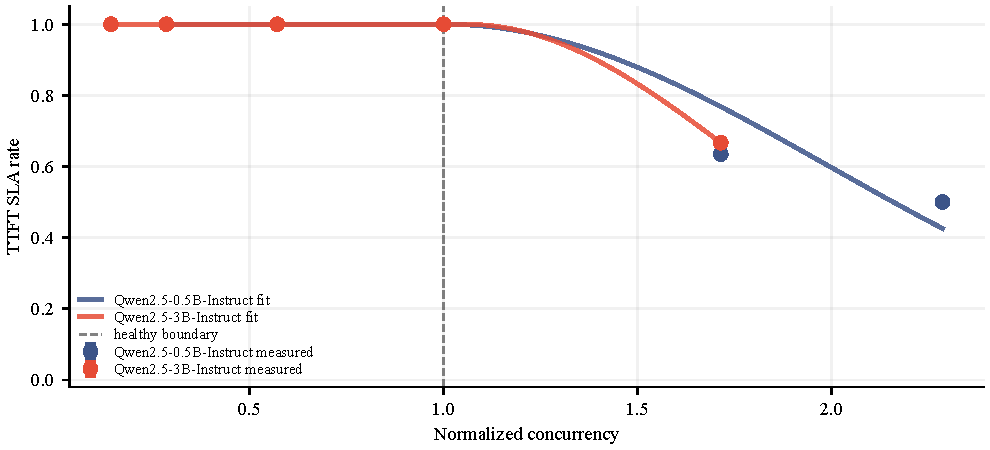
\includegraphics[width=0.88\textwidth]{vllm_qos_anchor.pdf}
\caption{Controlled vLLM single-GPU overload measurements used as QoS degradation anchors. The x-axis is concurrency normalized by the largest healthy concurrency level, and the y-axis is the SLA attainment rate for a 0.5-second TTFT threshold. Points are means over five repeated measurements; lines are fitted threshold-type QoS functions.}
\label{fig:vllm_qos_anchor}
\end{figure}

\section{Results}
\label{sec:results}

\subsection{Uncongested regime: demand shifts but profit effects remain limited}

With baseline capacity, the market is not congested: peak utilization under uniform pricing is only $0.213$, and QoS remains equal to one. Table~\ref{tab:uncongested} compares uniform pricing with time-of-use dynamic pricing.

\begin{table}[H]
\centering
\caption{Uncongested regime: uniform pricing versus dynamic pricing under deterministic grid search}
\label{tab:uncongested}
\begin{tabular}{lcc}
\toprule
Metric & Uniform pricing & Dynamic pricing \\
\midrule
System profit & 1193.3 & 1139.4 \\
Peak utilization & 0.213 & 0.261 \\
Elastic-demand centroid shift & \multicolumn{2}{c}{$+0.177$} \\
Rigid-demand centroid shift & \multicolumn{2}{c}{$+0.077$} \\
\bottomrule
\end{tabular}
\end{table}

The demand-shifting pattern is stable. Under dynamic pricing, the centroid of time-flexible demand shifts by $+0.177$ periods, whereas the centroid of time-rigid demand shifts by $+0.077$ periods. The shift of time-flexible demand is about $2.3$ times as large as that of time-rigid demand, which matches the intended response pattern. Because QoS is already one in the uncongested regime, however, there is little scope for quality improvement. The profit effect is neutral to mildly negative: across the elastic-population scan, the gains are $0\%$, $-0.32\%$, $-4.51\%$, $-3.76\%$, and $-3.00\%$. Time-of-use pricing becomes useful for QoS protection only when the market enters congestion.

\subsection{Congested regime: QoS evidence strengthens, whereas profit remains unstable}

After capacity is tightened, uniform pricing pushes the market into congestion. Table~\ref{tab:congested} reports four objects: the uniform-pricing baseline, the dynamic coarse-grid time-averaged strategy, the dynamic fine-grid pure snapshot, and the finite-grid mixed-strategy check. Table~\ref{tab:evidence_boundary} then states how each object is used in the paper's claim structure. This comparison separates conclusions that depend on solver resolution from those that remain valid under the lower-exploitability finite-grid mixed profile.

\begin{table}[H]
\centering
\caption{Congested regime: uniform pricing versus dynamic pricing under time-averaged, snapshot, and mixed-strategy checks}
\label{tab:congested}
\small
\begin{tabular}{lcccc}
\toprule
Metric & Uniform pricing & Dynamic coarse grid & Dynamic fine snapshot & Mixed check \\
\midrule
Peak utilization & 0.782 & 0.706 & 0.666 & 0.703 \\
Minimum QoS & 0.756 & 0.968 & 0.990 & 0.970 \\
System profit & 1783 & 1949 & 1749 & 1733 \\
Profit change & --- & $+9.3\%$ & $-1.9\%$ & $-2.8\%$ \\
Maximum regret & --- & 4.98 & 22.30 & 0.203 \\
\bottomrule
\end{tabular}
\end{table}

\begin{table}[H]
\centering
\caption{Evidence boundary for the congested regime}
\label{tab:evidence_boundary}
\small
\begin{tabular}{p{0.25\textwidth}p{0.30\textwidth}p{0.35\textwidth}}
\toprule
Object & Solver status & Claim supported in this paper \\
\midrule
Uniform-pricing baseline & Fictitious play reaches the criterion within 10 rounds & Used as the congested baseline. \\
Dynamic coarse grid & Regret is $4.98$ after 22 rounds, but the coarse grid may hide finer deviations & Used as a low-resolution diagnostic; not used alone to support a quantitative profit conclusion. \\
Dynamic fine-grid snapshot & Maximum regret is approximately $22.3$ after 40 rounds, above the $<5$ criterion & Used only as a resolution stress test and directional comparison; not interpreted as a pure-strategy equilibrium. \\
Finite-grid mixed diagnostic & Full 225-point fine-grid scan gives maximum regret $0.203$ & Supports the QoS result for the finite-grid mixed/averaged profile; not extrapolated to the continuous strategy space. \\
\bottomrule
\end{tabular}
\end{table}

\begin{figure}[H]
\centering
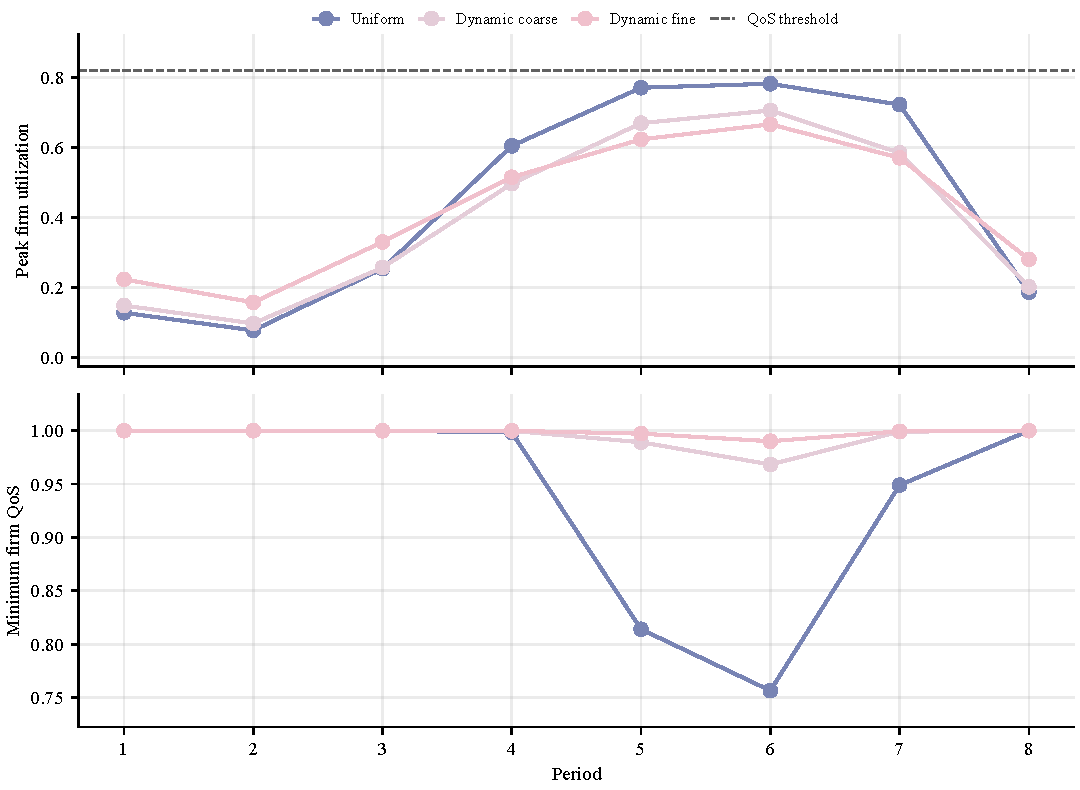
\includegraphics[width=0.86\textwidth]{qos_utilization_profiles.pdf}
\caption{Period-level utilization and QoS profiles in the congested regime. The dynamic strategies lower peak utilization and raise the minimum provider QoS in both coarse-grid and fine-grid snapshots. The dashed line in the utilization panel marks the utilization threshold at which QoS degradation begins.}
\label{fig:qos_profiles}
\end{figure}

\begin{figure}[H]
\centering
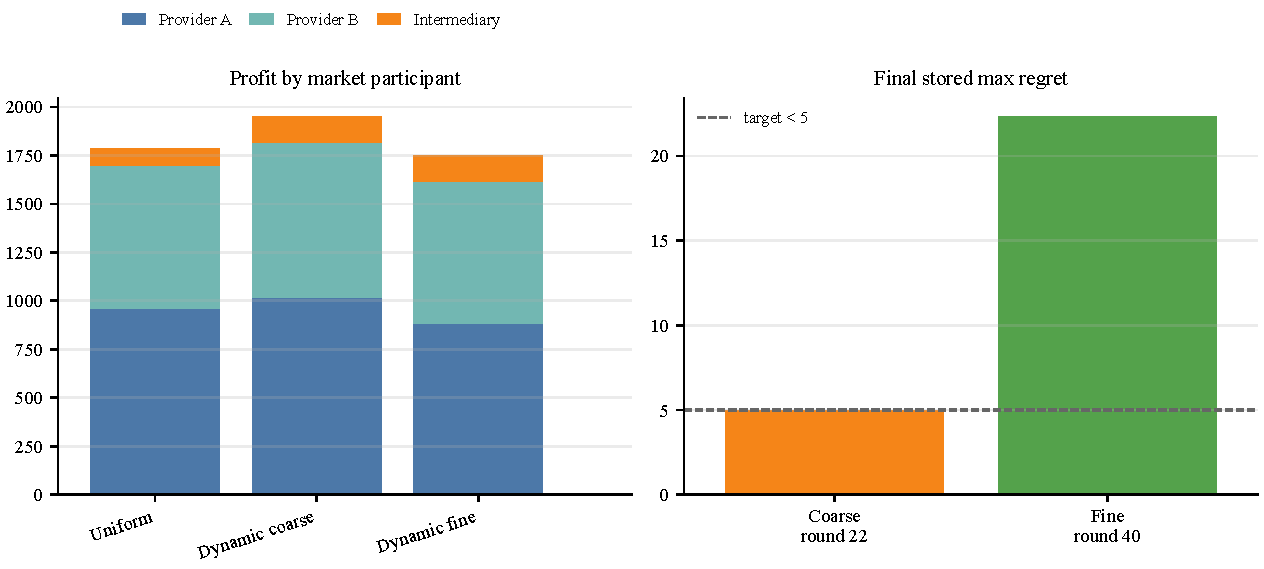
\includegraphics[width=0.88\textwidth]{profit_components_and_regret.pdf}
\caption{Profit components and pure-strategy regret boundary. The left panel decomposes profit by market participant (Provider A, Provider B, and the intermediary), and the right panel reports stored best-response regret. The coarse snapshot reaches regret $<5$, whereas the fine-grid pure snapshot remains at $22.3$ and is used only as a resolution stress test.}
\label{fig:profit_regret}
\end{figure}

\begin{figure}[H]
\centering
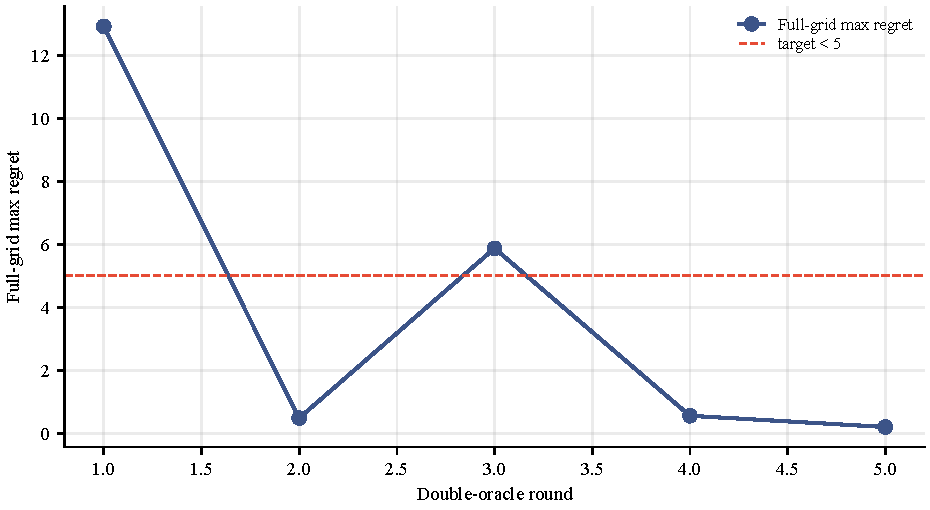
\includegraphics[width=0.76\textwidth]{mixed_oracle_regret.pdf}
\caption{Double-oracle finite-grid mixed-strategy diagnostic. Each round adds the best deviation against the current mixed profile on the complete 225-point fine grid. The fifth round obtains a $5\times5$ support profile, and full-grid maximum regret falls to $0.203$.}
\label{fig:mixed_oracle}
\end{figure}

Figures~\ref{fig:qos_profiles}, \ref{fig:profit_regret}, and \ref{fig:mixed_oracle} visualize the same evidence from the period, profit-component, and regret perspectives. The QoS-improvement direction holds for both snapshots and the mixed profile. Uniform pricing lowers the minimum QoS to $0.756$ and raises peak utilization to $0.782$. The dynamic pricing snapshots reduce peak utilization to the $0.66$--$0.71$ range and raise minimum QoS to the $0.97$--$0.99$ range. The finite-grid mixed profile has expected peak utilization $0.703$ and minimum QoS $0.970$. The QoS result is not driven solely by the high-regret fine-grid pure snapshot; it is also supported by a low-regret finite-grid mixed/averaged profile.

No stable positive profit effect is observed. System profit increases by $+9.3\%$ in the coarse-grid snapshot, decreases by $-1.9\%$ in the fine-grid snapshot, and decreases by approximately $-2.8\%$ in the low-regret mixed profile. The paper does not report profit improvement as a positive finding. Within the current solution budget and pricing-shape family, time-of-use pricing has QoS-protection value but does not provide evidence of a reliable positive profit gain.

The provider-heterogeneity hypothesis is also not stable. A natural conjecture is that the smaller-capacity provider would rely more heavily on dynamic pricing, implying $\delta_B>\delta_A$. The coarse grid gives $\delta_A=0.383$ and $\delta_B=0.023$, whereas the fine grid gives $\delta_A=0.059$ and $\delta_B=0.278$. The direction reverses with grid resolution, so the paper does not retain a claim about which provider prices more dynamically. The asymmetry in demand shifting is similarly clear in the uncongested regime but weak under the congested solution objects: in the fine-grid case, the centroids of elastic and rigid demand are $4.23$ and $4.31$, respectively, leaving little separation.

\subsection{SMPT baseline diagnostics and structural checks}

Uniform pricing is a useful baseline, but it may be too weak on its own. To test whether the QoS result is only a uniform-baseline artifact, four service-management baselines are added around the congested setting. They are off-peak discount only, peak surcharge only, dynamic coarse pricing with fixed equal routing, and an admission-control check. Table~\ref{tab:smpt_baselines} reports these baselines next to the static candidate response and the two main dynamic snapshots.

\begin{table}[H]
\centering
\caption{SMPT baseline diagnostics in the congested setting}
\label{tab:smpt_baselines}
\small
\begin{tabular}{lcccc}
\toprule
Policy or diagnostic & Peak util. & Min QoS & Profit change & Served volume \\
\midrule
Static pricing with QoS routing & 0.782 & 0.756 & --- & 2610 \\
Off-peak discount only & 0.766 & 0.833 & $+5.0\%$ & 2849 \\
Peak surcharge only & 0.738 & 0.921 & $+5.8\%$ & 2672 \\
Dynamic coarse & 0.706 & 0.968 & $+9.3\%$ & 2865 \\
Dynamic fine snapshot & 0.666 & 0.990 & $-1.9\%$ & 3043 \\
Dynamic coarse with equal routing & 0.753 & 0.881 & $+5.9\%$ & 2817 \\
\bottomrule
\end{tabular}
\end{table}

The one-sided price-shape baselines improve QoS, but neither reaches the full dynamic coarse snapshot. Off-peak discounts increase served volume but leave more peak pressure than the full dynamic shape. Peak surcharges reduce peak utilization more directly but recover less served volume. Equal routing still improves on the static baseline, yet it leaves minimum QoS at $0.881$ rather than $0.968$, indicating that both price timing and QoS-aware routing contribute to the reported result. Matching the dynamic coarse peak utilization with a uniform-price admission-control check would require admitting as little as $90.2\%$ of demand in the tightest period and $97.4\%$ on average. This check is not a profit comparison, but it shows the service-quality cost of reaching a similar peak-utilization target by throttling rather than pricing.

\begin{table}[H]
\centering
\caption{Structural ablations for the dynamic coarse policy}
\label{tab:structural_ablations}
\small
\begin{tabular}{lccc}
\toprule
Ablation variant & Min-QoS gain & Peak-util. reduction & Profit change \\
\midrule
Baseline model & $+0.212$ & $+0.076$ & $+9.3\%$ \\
No outside option & $+0.307$ & $+0.067$ & $+11.3\%$ \\
Suppressed direct-provider channel & $+0.000$ & $+0.209$ & $+0.0\%$ \\
Homogeneous capacity & $-0.054$ & $-0.154$ & $-3.6\%$ \\
No time-flexible users & $+0.155$ & $+0.046$ & $+6.1\%$ \\
Fixed equal routing & $+0.125$ & $+0.029$ & $+5.9\%$ \\
\bottomrule
\end{tabular}
\end{table}

Table~\ref{tab:structural_ablations} narrows the mechanism claim. The dynamic coarse policy keeps a material positive QoS gain in four ablation rows. Two boundary cases are especially informative. Suppressing the direct-provider channel makes both policies nearly uncongested, so the dynamic advantage almost disappears. Equalizing provider capacity reverses the advantage, with QoS gain $-0.054$ and profit change $-3.6\%$. The result is strongest when the market has heterogeneous capacity, direct-provider alternatives, and congestion severe enough for prices to matter.

\subsection{Local parameter stress tests}

To examine whether the QoS direction depends on a single synthetic calibration, four groups of local perturbations are evaluated around the congested baseline: capacity scale, price sensitivity, switching cost, and the QoS threshold. At each perturbation point, the reported uniform, dynamic coarse-grid, and dynamic fine-grid policy snapshots are evaluated without re-solving the game. The exercise is a fixed-policy stress test, not a cross-parameter equilibrium statement.

\begin{figure}[H]
\centering
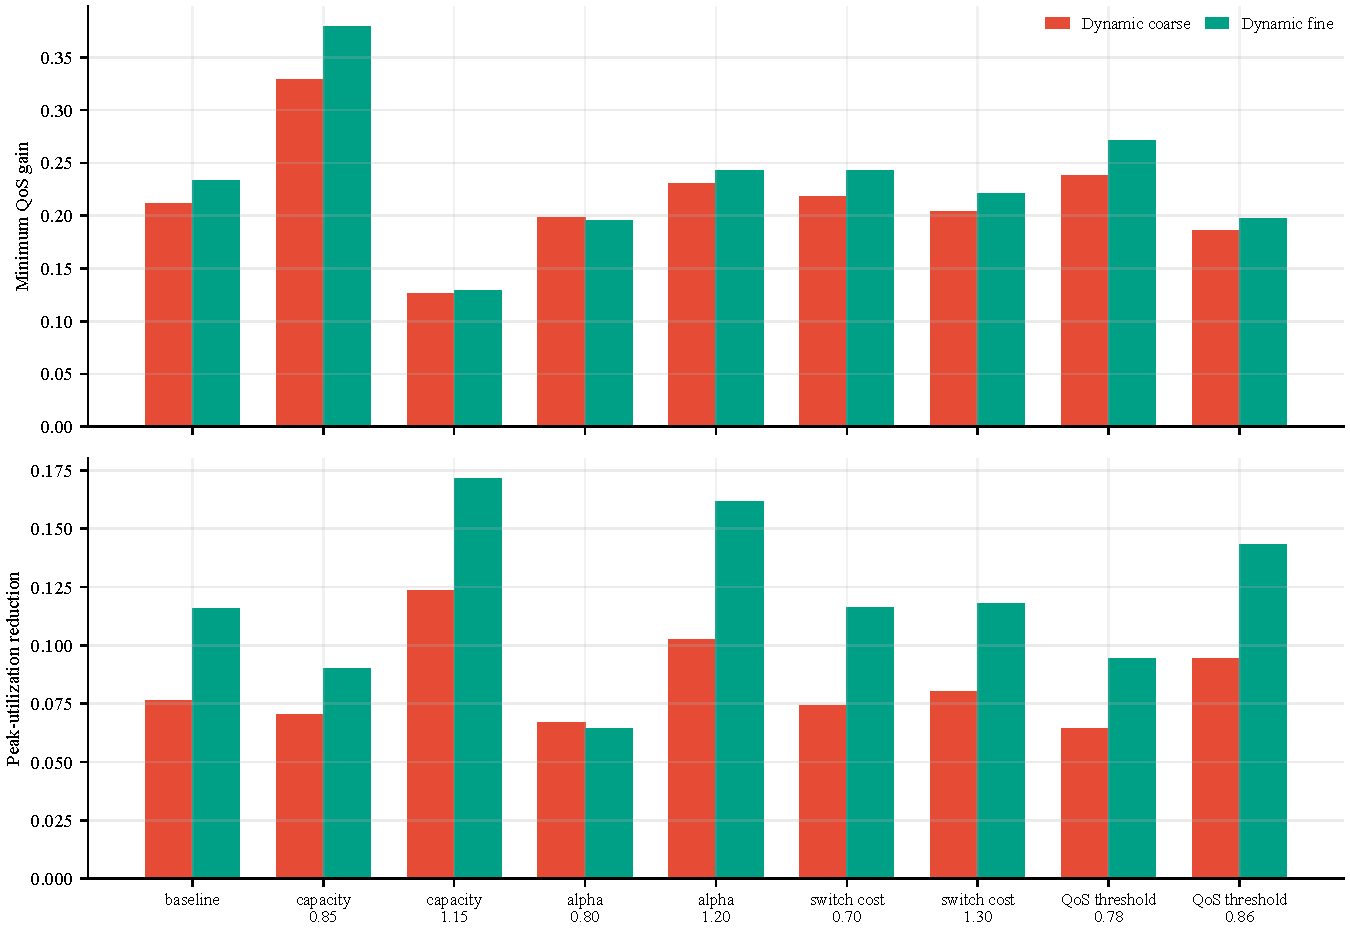
\includegraphics[width=0.92\textwidth]{parameter_sweep_qos.pdf}
\caption{Parameter stress tests. Across nine perturbation scenarios, the dynamic coarse-grid and dynamic fine-grid snapshots maintain positive minimum-QoS gains and lower peak utilization relative to uniform pricing.}
\label{fig:parameter_sweep}
\end{figure}

Figure~\ref{fig:parameter_sweep} shows that both dynamic snapshots preserve positive QoS gains and lower peak utilization across all nine perturbation scenarios. The smallest minimum-QoS gain is $0.126$ for the coarse-grid snapshot and $0.129$ for the fine-grid snapshot. Profit remains unsuitable for a strong positive conclusion: the coarse-grid snapshot is profitable in all nine scenarios, whereas the fine-grid snapshot is profitable in only one. This scan supports local fixed-policy robustness of the QoS direction while again showing that profit improvement is not robust.

\begin{figure}[H]
\centering
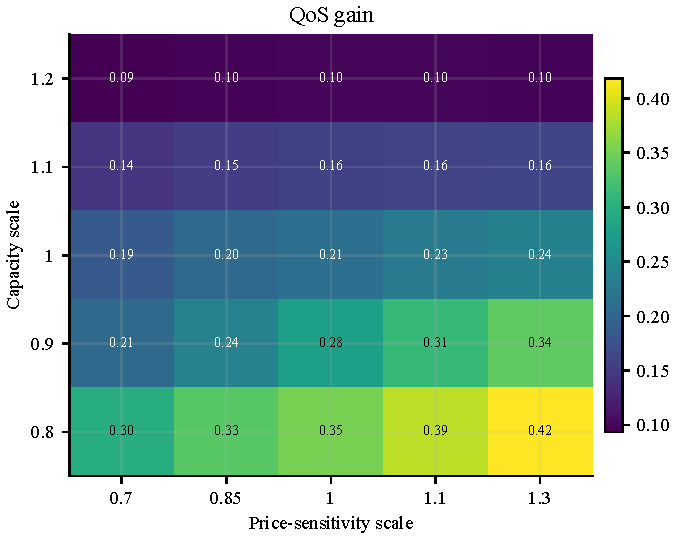
\includegraphics[width=0.48\textwidth]{smpt_phase_qos_gain.pdf}
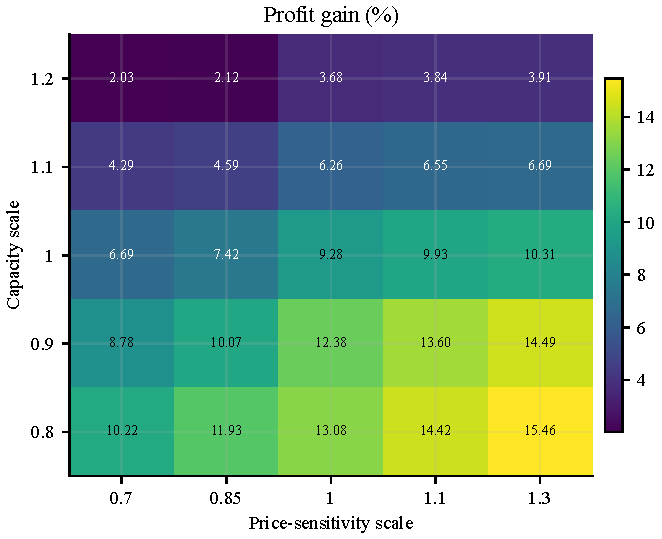
\includegraphics[width=0.48\textwidth]{smpt_phase_profit_gain.pdf}
\caption{Fixed-policy phase grid over capacity scale and price-sensitivity scale. The dynamic coarse policy keeps positive QoS gains and peak-utilization reductions in all 25 grid points. Profit is positive on this fixed-policy grid, but the restricted re-solved sensitivity in Table~\ref{tab:resolved_sensitivity} remains mixed.}
\label{fig:smpt_phase}
\end{figure}

The fixed-policy phase grid in Figure~\ref{fig:smpt_phase} gives a broader local view. QoS gain and peak-utilization reduction are positive in all 25 capacity--elasticity grid points, with minimum QoS gain $0.094$. Profit is positive on this fixed-policy coarse-policy grid, ranging from $+2.0\%$ to $+15.5\%$. This does not overturn the profit-boundary result because the coarse policy is held fixed.

\begin{table}[H]
\centering
\caption{Restricted local re-solve under selected perturbations}
\label{tab:resolved_sensitivity}
\small
\begin{tabular}{lccc}
\toprule
Scenario & Min-QoS gain & Peak-util. reduction & Profit change \\
\midrule
Capacity scale $0.90$ & $+0.280$ & $+0.060$ & $+12.5\%$ \\
Price sensitivity scale $1.15$ & $+0.241$ & $+0.150$ & $-1.4\%$ \\
Flexible-user share $0.70$ & $+0.242$ & $+0.136$ & $-1.9\%$ \\
QoS threshold $0.78$ & $+0.241$ & $+0.066$ & $+11.0\%$ \\
Outside-option utility $0.50$ & $+0.156$ & $+0.069$ & $+0.7\%$ \\
\bottomrule
\end{tabular}
\end{table}

For this stronger check, the local candidate set contains the static, dynamic coarse, dynamic fine, off-peak-only, and peak-only shapes, and each scenario runs four local best-response rounds. Table~\ref{tab:resolved_sensitivity} keeps positive QoS gain in all five rows, with gains between $0.156$ and $0.280$. Profit remains mixed. This is the strongest current evidence for the paper's central separation: QoS protection is easier to reproduce than profit improvement.

\section{Discussion: QoS Improvement and the Profit Boundary}
\label{sec:discussion}

The central finding in the congested regime is that QoS improves substantially, rising from $0.756$ to approximately $0.97$ or higher, whereas profit does not show a stable positive response. Because the sign of the profit effect changes across the coarse-grid snapshot, the fine-grid snapshot, and the low-regret mixed profile, profit is not treated as a positive result. It is used instead to explain why QoS improvement does not necessarily translate into provider profit.

\begin{figure}[H]
\centering
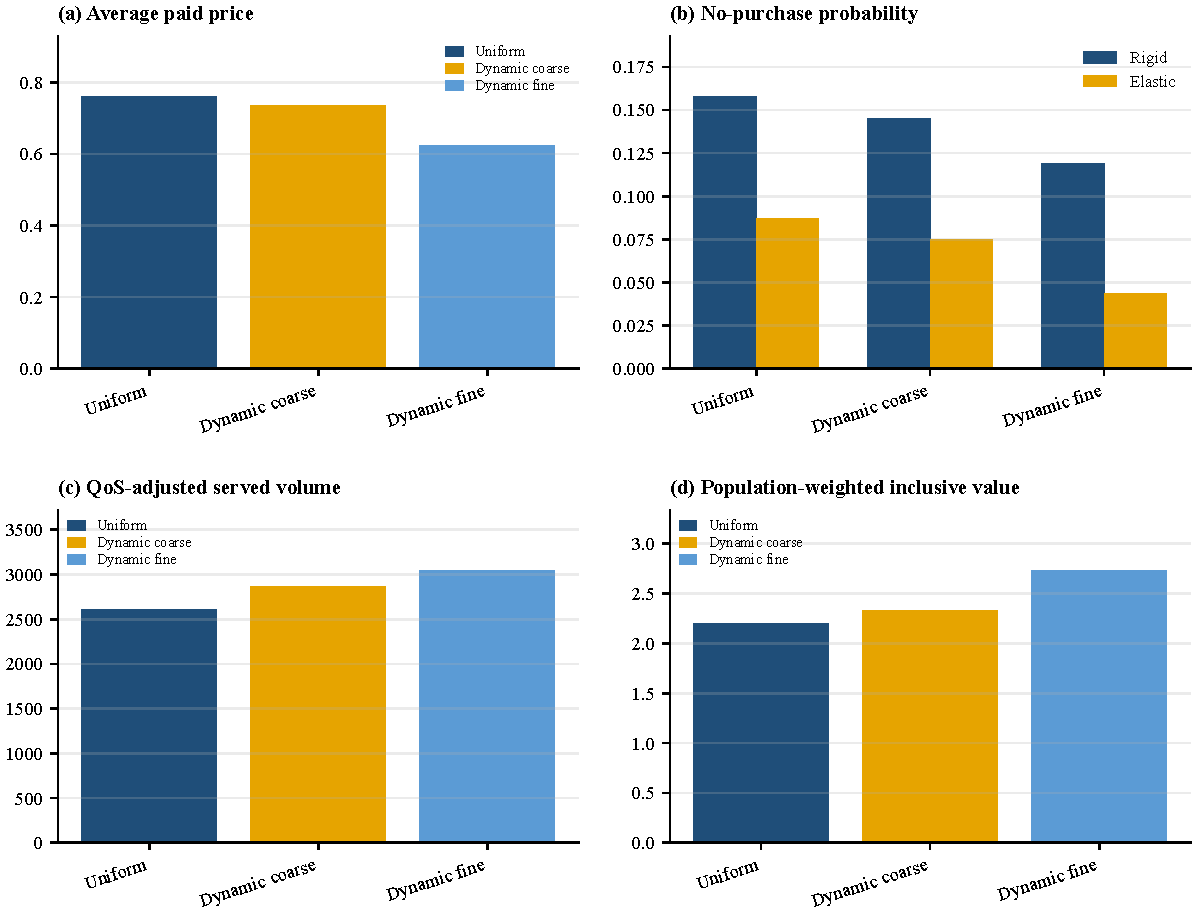
\includegraphics[width=0.9\textwidth]{mechanism_diagnostics.pdf}
\caption{Mechanism diagnostics in the congested regime. Panels (a)--(d) report average paid price, no-purchase probability, QoS-adjusted served volume, and population-weighted inclusive value, respectively. Dynamic pricing improves served-volume and no-purchase outcomes while lowering average paid price, consistent with surplus reallocation rather than a stable provider-profit gain.}
\label{fig:mechanism}
\end{figure}

\subsection{Surplus reallocation rather than additional supply}

Fixed capacity is the central constraint in this simulation. Time-of-use pricing cannot add physical GPU supply; it can only change the distribution of demand across periods and channels. The patterns in Figure~\ref{fig:mechanism} are consistent with this interpretation. Under the uniform congested baseline, QoS-adjusted served volume is $2610$. Under the dynamic coarse-grid and fine-grid snapshots, it increases to $2865$ and $3043$, respectively. At the same time, the exit probability of time-rigid users falls from $0.158$ to $0.145/0.119$, and the exit probability of time-flexible users falls from $0.087$ to $0.075/0.044$. These values show that dynamic pricing recovers part of the service loss caused by congestion. The mixed-strategy check also indicates that this QoS direction is not dependent on a single high-regret fine-grid point.

The recovered service volume, however, is not converted into stable profit. The main reason is that price and quantity move in opposite directions: the average paid price declines from $0.761$ to $0.735/0.625$. For providers, the positive forces include higher peak-period margins, better use of idle off-peak capacity, and increased effective billed volume as QoS recovers. Negative forces operate at the same time. Peak-period price increases can shift price-sensitive demand to a rival, a direct option, or the outside option. Off-peak discounts reduce per-request margins. Flexible users displaced from the peak may also become net lost demand. Peak-price gains may be offset by demand loss, and additional off-peak volume may be offset by lower margins.

This pattern should not be read as a theorem under fixed total demand. The model includes an outside option and a price-responsive market-size term, so internal demand changes with both price and QoS. A more accurate interpretation is surplus reallocation. Time-of-use pricing primarily reallocates demand across time and channels, rather than reliably creating new surplus that can be fully captured by providers.

\subsection{Why recovered QoS losses do not reliably become profit}

A return of QoS from $0.756$ to above $0.97$ means that fewer requests are lost to congestion-related service degradation. Intuitively, this recovery might be expected to increase profit. Two forces weaken that conversion. First, peak shaving itself requires some peak demand to move, switch channels, or exit. To reduce utilization from approximately $0.78$ to the $0.66$--$0.71$ range, part of the high-peak demand must be displaced. The effective billed volume recovered through better QoS can be offset by lower prices and demand reallocation. Second, competition and the outside option restrict price increases. Because two heterogeneous providers compete and users can buy directly or exit, no provider can fully appropriate the value of QoS improvement. Some of the surplus is more likely to appear as better user experience, higher completion, or lower prices under competition, rather than as a stable increase in provider profit.

\subsection{Operational and regulatory implications}

Dynamic pricing and surge pricing are often interpreted as revenue instruments during congestion. The present simulation results support a more cautious interpretation. In an inference-service market with fixed capacity, provider competition, and user exit, time-of-use pricing is better understood as a QoS-protection instrument. Within the current model and solution budget, it does not provide strong evidence of profit improvement. For regulators, evaluation of time-of-use pricing should consider not only whether prices rise during peak periods, but also whether congestion and failed service are reduced. For operators, the stronger operational justification is service-level management, not reliable revenue growth.

\section{Limitations}
\label{sec:limitations}

Several limitations should be made explicit. All economic parameters, including price sensitivity, switching cost, capacity cost, the elastic-user population share, and outside-option utility, are synthetic calibrations. Real request traces are not used for calibration. The reported percentage changes indicate mechanism direction rather than production forecasts. Public API prices provide only an order-of-magnitude price reference, and controlled vLLM single-GPU measurements provide only a QoS-shape reference. Neither replaces real arrival processes, long-context workloads, multi-model or multi-GPU measurements, production completion curves, or user price-elasticity estimates.

The solution evidence is also bounded. Provider strategies are restricted to a low-dimensional pricing-shape family; the paper does not claim a global optimum in the continuous strategy space. The fine-grid pure snapshot remains high-regret and cannot be interpreted as a pure-strategy equilibrium. The double-oracle check reduces regret to $0.203$ on the finite 225-point grid, but it remains a mixed/averaged strategy result over a finite candidate set, not a global equilibrium result in the continuous strategy space. The nine-scenario stress test and the 25-point phase grid evaluate already reported policy snapshots under perturbed parameters rather than re-solving the game at every point. The restricted local re-solve is stronger, but it uses a small candidate set and four best-response rounds. The QoS-improvement direction is retained with greater confidence than any conclusion about profit, provider-specific dynamic intensity, or continuous-space equilibrium properties.

The scope is further limited by market structure and backend measurement. The paper studies two providers and one intermediary. Interactions among more providers, multiple intermediaries, long-term capacity contracts, and model routing are outside the current model. QoS degradation is represented by a synthetic sigmoid curve whose shape is anchored by controlled measurements; real backend completion and latency curves would need to be recalibrated using controlled production-like measurements or operational traces. Finally, the absence of a robust positive profit gain depends on the present fixed-capacity, competitive, and demand assumptions. The conclusion could change if total demand were more price-responsive or if capacity were adjustable in the short run.

\section{Conclusion}
\label{sec:conclusion}

This paper studied whether time-of-use dynamic pricing can improve the QoS of inference services under fixed GPU capacity. A market-level simulation model was developed with two heterogeneous competing providers, one routing intermediary, two user types, and an outside option. Provider pricing was restricted to a low-dimensional time-shape family, and provider competition was approximated through fictitious play. This approach mitigated the limit-cycle behaviour observed under naive best responses in the congested regime and made the simulation process reproducible and diagnostically transparent.

Across coarse-grid and fine-grid snapshots, a finite-grid mixed-strategy check, service-management baselines, structural ablations, local stress tests, a phase grid, and restricted local re-solves, the results support a bounded but consistent QoS conclusion. Under congestion, time-of-use pricing reduces peak load and raises minimum QoS from $0.756$ to approximately $0.97$ or above. The double-oracle check reduces maximum regret to $0.203$ on the complete 225-point fine grid, and the additional SMPT checks show that QoS gains are easier to reproduce than profit gains. Profit results are not stable: the sign of the profit effect changes across solver objects and grid resolutions. The paper does not claim that time-of-use pricing reliably increases profit. Instead, the results suggest surplus reallocation. Under fixed capacity, competition, and user exit, price changes can recover congestion losses and reduce exit, but the benefits may be offset by demand outflow, thinner margins, and surplus transfer. For operators and regulators, time-of-use pricing is better viewed as a service-quality management instrument than as a reliable revenue-growth tool. Future work should incorporate real trace calibration, verify low exploitability over larger or continuous strategy spaces, and extend the model to additional providers and intermediaries.

\section*{Reproducibility, Data Availability, and Artifact Boundary}

The peak-shaving simulation modules are \path{pricing_sim/peak_shaving_config.py},
\path{pricing_sim/peak_shaving_market.py}, and
\path{pricing_sim/peak_shaving_equilibrium.py}. The main experiment entry points are:
\begin{itemize}[leftmargin=2em]
  \item \path{experiments/run_peak_shaving_experiments.py}: uncongested main experiment;
  \item \path{experiments/run_peak_shaving_congested_fp.py}: congested fictitious play;
  \item \path{experiments/run_fp_dynamic_converge.py}: regret convergence and checkpoint continuation;
  \item \path{experiments/run_peak_shaving_robustness.py}: QoS shape, outside-option, and cross-seed checks;
  \item \path{experiments/run_peak_shaving_mixed_oracle.py}: finite-grid mixed-strategy diagnostic;
  \item \path{experiments/run_peak_shaving_parameter_sweep.py}: local parameter stress tests;
  \item \path{experiments/run_peak_shaving_smpt_experiments.py}: SMPT baselines, ablations, phase grid, restricted local re-solve, and fixed-point residual diagnostics;
  \item \path{experiments/run_peak_shaving_smpt_vv_audit.py}: initialization and damping-factor fixed-point audit;
  \item \path{experiments/build_peak_shaving_measurement_anchor.py}: controlled vLLM QoS-shape anchor.
\end{itemize}
Mechanism diagnostics and figures are rebuilt from existing strategy artifacts by
\path{experiments/build_peak_shaving_diagnostics.py}. Machine-readable artifacts are stored under
\path{artifacts/peak_shaving/}, with subdirectories \path{20260618/}, \path{20260619/},
\path{20260619_submission/}, and \path{20260619_smpt/}. Figures are stored under \path{figures/}, with subdirectories
\path{peak_shaving_diagnostics/}, \path{peak_shaving_submission/}, and \path{peak_shaving_smpt/}. Parameter values, grid definitions, artifact mappings, and reproduction commands are provided in the supplementary file
\path{peak_shaving_dynamic_pricing_sci_en_supplement_2026-06-19.tex}.

A public project repository containing the current manuscript, code, figure scripts, and generated artifacts is available at \url{https://github.com/cccht/paper_token_price}. A versioned GitHub release for this submission candidate is available at \url{https://github.com/cccht/paper_token_price/releases/tag/smpt-submission-candidate-2026-06-21}. If a persistent archival identifier is required, this release should be mirrored to an archival service such as Zenodo or OSF before formal submission. Until such a digital object identifier is created, the GitHub release should be treated as a versioned reproducibility package rather than a persistent data identifier.

\section*{Declaration of Generative AI and AI-Assisted Technologies}

During manuscript preparation, AI-assisted tools were used for language polishing, consistency checks, and internal reviewer-style checks. The authors remain responsible for the simulation model, experimental artifacts, numerical results, interpretation, and final text.

\small
\bibliographystyle{unsrtnat}
\bibliography{verified_refs}

\end{document}

% Polishing notes (not compiled):
% - Rewritten into formal academic English for Simulation Modelling Practice and Theory.
% - Terminology standardized: simulation model, modelling, verification, validation anchor, QoS, API, GPU, LLM, TTFT, SLA.
% - Abstract compressed to the SMPT 250-word limit and keywords reduced to seven journal-appropriate terms.
% - Section titles and transitions refined to emphasize simulation-modelling contribution, validation anchors, finite-grid diagnostics, and bounded evidence.
% - Grammar, style, tense, voice, paragraph flow, captions, and table labels polished without changing formulas, numerical results, citations, or bibliography commands.
